\documentclass[twoside]{book}

% Packages required by doxygen
\usepackage{calc}
\usepackage{doxygen}
\usepackage{graphicx}
\usepackage[utf8]{inputenc}
\usepackage{makeidx}
\usepackage{multicol}
\usepackage{multirow}
\usepackage{textcomp}
\usepackage[table]{xcolor}

% Font selection
\usepackage[T1]{fontenc}
\usepackage{mathptmx}
\usepackage[scaled=.90]{helvet}
\usepackage{courier}
\usepackage{amssymb}
\usepackage{sectsty}
\renewcommand{\familydefault}{\sfdefault}
\allsectionsfont{%
  \fontseries{bc}\selectfont%
  \color{darkgray}%
}
\renewcommand{\DoxyLabelFont}{%
  \fontseries{bc}\selectfont%
  \color{darkgray}%
}

% Page & text layout
\usepackage{geometry}
\geometry{%
  a4paper,%
  top=2.5cm,%
  bottom=2.5cm,%
  left=2.5cm,%
  right=2.5cm%
}
\tolerance=750
\hfuzz=15pt
\hbadness=750
\setlength{\emergencystretch}{15pt}
\setlength{\parindent}{0cm}
\setlength{\parskip}{0.2cm}
\makeatletter
\renewcommand{\paragraph}{%
  \@startsection{paragraph}{4}{0ex}{-1.0ex}{1.0ex}{%
    \normalfont\normalsize\bfseries\SS@parafont%
  }%
}
\renewcommand{\subparagraph}{%
  \@startsection{subparagraph}{5}{0ex}{-1.0ex}{1.0ex}{%
    \normalfont\normalsize\bfseries\SS@subparafont%
  }%
}
\makeatother

% Headers & footers
\usepackage{fancyhdr}
\pagestyle{fancyplain}
\fancyhead[LE]{\fancyplain{}{\bfseries\thepage}}
\fancyhead[CE]{\fancyplain{}{}}
\fancyhead[RE]{\fancyplain{}{\bfseries\leftmark}}
\fancyhead[LO]{\fancyplain{}{\bfseries\rightmark}}
\fancyhead[CO]{\fancyplain{}{}}
\fancyhead[RO]{\fancyplain{}{\bfseries\thepage}}
\fancyfoot[LE]{\fancyplain{}{}}
\fancyfoot[CE]{\fancyplain{}{}}
\fancyfoot[RE]{\fancyplain{}{\bfseries\scriptsize Generated on Sat Apr 12 2014 23:03:18 for SDLGame by Doxygen }}
\fancyfoot[LO]{\fancyplain{}{\bfseries\scriptsize Generated on Sat Apr 12 2014 23:03:18 for SDLGame by Doxygen }}
\fancyfoot[CO]{\fancyplain{}{}}
\fancyfoot[RO]{\fancyplain{}{}}
\renewcommand{\footrulewidth}{0.4pt}
\renewcommand{\chaptermark}[1]{%
  \markboth{#1}{}%
}
\renewcommand{\sectionmark}[1]{%
  \markright{\thesection\ #1}%
}

% Indices & bibliography
\usepackage{natbib}
\usepackage[titles]{tocloft}
\setcounter{tocdepth}{3}
\setcounter{secnumdepth}{5}
\makeindex

% Hyperlinks (required, but should be loaded last)
\usepackage{ifpdf}
\ifpdf
  \usepackage[pdftex,pagebackref=true]{hyperref}
\else
  \usepackage[ps2pdf,pagebackref=true]{hyperref}
\fi
\hypersetup{%
  colorlinks=true,%
  linkcolor=blue,%
  citecolor=blue,%
  unicode%
}

% Custom commands
\newcommand{\clearemptydoublepage}{%
  \newpage{\pagestyle{empty}\cleardoublepage}%
}


%===== C O N T E N T S =====

\begin{document}

% Titlepage & ToC
\hypersetup{pageanchor=false}
\pagenumbering{roman}
\begin{titlepage}
\vspace*{7cm}
\begin{center}%
{\Large S\-D\-L\-Game }\\
\vspace*{1cm}
{\large Generated by Doxygen 1.8.4}\\
\vspace*{0.5cm}
{\small Sat Apr 12 2014 23:03:18}\\
\end{center}
\end{titlepage}
\clearemptydoublepage
\tableofcontents
\clearemptydoublepage
\pagenumbering{arabic}
\hypersetup{pageanchor=true}

%--- Begin generated contents ---
\chapter{Hierarchical Index}
\section{Class Hierarchy}
This inheritance list is sorted roughly, but not completely, alphabetically\-:\begin{DoxyCompactList}
\item \contentsline{section}{class}{\pageref{classclass}}{}
\item \contentsline{section}{Doxy\-Class}{\pageref{class_doxy_class}}{}
\item \contentsline{section}{L\-Engine}{\pageref{class_l_engine}}{}
\item \contentsline{section}{L\-Object}{\pageref{class_l_object}}{}
\begin{DoxyCompactList}
\item \contentsline{section}{L\-Game\-Base}{\pageref{class_l_game_base}}{}
\begin{DoxyCompactList}
\item \contentsline{section}{Game\-One}{\pageref{class_game_one}}{}
\end{DoxyCompactList}
\end{DoxyCompactList}
\item \contentsline{section}{S\-D\-L\-Renderer}{\pageref{class_s_d_l_renderer}}{}
\item \contentsline{section}{S\-D\-L\-Window}{\pageref{class_s_d_l_window}}{}
\end{DoxyCompactList}

\chapter{Class Index}
\section{Class List}
Here are the classes, structs, unions and interfaces with brief descriptions\-:\begin{DoxyCompactList}
\item\contentsline{section}{\hyperlink{classclass}{class} \\*\mbox{[}brief description\mbox{]} }{\pageref{classclass}}{}
\item\contentsline{section}{\hyperlink{class_doxy_class}{Doxy\-Class} }{\pageref{class_doxy_class}}{}
\item\contentsline{section}{\hyperlink{class_game_one}{Game\-One} }{\pageref{class_game_one}}{}
\item\contentsline{section}{\hyperlink{class_l_engine}{L\-Engine} }{\pageref{class_l_engine}}{}
\item\contentsline{section}{\hyperlink{class_l_game_base}{L\-Game\-Base} }{\pageref{class_l_game_base}}{}
\item\contentsline{section}{\hyperlink{class_l_object}{L\-Object} }{\pageref{class_l_object}}{}
\item\contentsline{section}{\hyperlink{class_s_d_l_renderer}{S\-D\-L\-Renderer} }{\pageref{class_s_d_l_renderer}}{}
\item\contentsline{section}{\hyperlink{class_s_d_l_window}{S\-D\-L\-Window} }{\pageref{class_s_d_l_window}}{}
\end{DoxyCompactList}

\chapter{File Index}
\section{File List}
Here is a list of all documented files with brief descriptions\-:\begin{DoxyCompactList}
\item\contentsline{section}{Source/include/{\bfseries Game\-One.\-h} }{\pageref{_game_one_8h}}{}
\item\contentsline{section}{Source/include/\hyperlink{_test_doxy_8h}{Test\-Doxy.\-h} }{\pageref{_test_doxy_8h}}{}
\item\contentsline{section}{Source/\-Libraries/\-L\-Engine/include/{\bfseries L\-Engine.\-h} }{\pageref{_l_engine_8h}}{}
\item\contentsline{section}{Source/\-Libraries/\-L\-Engine/include/{\bfseries L\-Game\-Base.\-h} }{\pageref{_l_game_base_8h}}{}
\item\contentsline{section}{Source/\-Libraries/\-L\-Engine/include/{\bfseries L\-Object.\-h} }{\pageref{_l_object_8h}}{}
\item\contentsline{section}{Source/\-Libraries/\-S\-D\-L\-Interface/include/{\bfseries S\-D\-L\-Event\-Loop.\-h} }{\pageref{_s_d_l_event_loop_8h}}{}
\item\contentsline{section}{Source/\-Libraries/\-S\-D\-L\-Interface/include/{\bfseries S\-D\-L\-Main.\-h} }{\pageref{_s_d_l_main_8h}}{}
\item\contentsline{section}{Source/\-Libraries/\-S\-D\-L\-Interface/include/{\bfseries S\-D\-L\-Renderer.\-h} }{\pageref{_s_d_l_renderer_8h}}{}
\item\contentsline{section}{Source/\-Libraries/\-S\-D\-L\-Interface/include/{\bfseries S\-D\-L\-Window.\-h} }{\pageref{_s_d_l_window_8h}}{}
\item\contentsline{section}{Source/\-Libraries/\-Util/include/{\bfseries types.\-h} }{\pageref{types_8h}}{}
\end{DoxyCompactList}

\chapter{Class Documentation}
\hypertarget{classclass}{\section{class Class Reference}
\label{classclass}\index{class@{class}}
}


\mbox{[}brief description\mbox{]}  




\subsection{Detailed Description}
\mbox{[}brief description\mbox{]} 

\mbox{[}detailed description\mbox{]}

\begin{DoxyAuthor}{Author}
\mbox{[}your name\mbox{]} 
\end{DoxyAuthor}
\begin{DoxyDate}{Date}
\mbox{[}the date\mbox{]} 
\end{DoxyDate}


The documentation for this class was generated from the following file\-:\begin{DoxyCompactItemize}
\item 
Source/include/\hyperlink{_test_doxy_8h}{Test\-Doxy.\-h}\end{DoxyCompactItemize}

\hypertarget{class_doxy_class}{\section{Doxy\-Class Class Reference}
\label{class_doxy_class}\index{Doxy\-Class@{Doxy\-Class}}
}
\subsection*{Public Member Functions}
\begin{DoxyCompactItemize}
\item 
int \hyperlink{class_doxy_class_a0e94b6dcef1700c34932ff689b3305a7}{Funtion} (int the\-Input\-Param)
\begin{DoxyCompactList}\small\item\em \mbox{[}brief description\mbox{]} \end{DoxyCompactList}\end{DoxyCompactItemize}


\subsection{Member Function Documentation}
\hypertarget{class_doxy_class_a0e94b6dcef1700c34932ff689b3305a7}{\index{Doxy\-Class@{Doxy\-Class}!Funtion@{Funtion}}
\index{Funtion@{Funtion}!DoxyClass@{Doxy\-Class}}
\subsubsection[{Funtion}]{\setlength{\rightskip}{0pt plus 5cm}int Doxy\-Class\-::\-Funtion (
\begin{DoxyParamCaption}
\item[{int}]{the\-Input\-Param}
\end{DoxyParamCaption}
)\hspace{0.3cm}{\ttfamily [inline]}}}\label{class_doxy_class_a0e94b6dcef1700c34932ff689b3305a7}


\mbox{[}brief description\mbox{]} 

\mbox{[}detailed description converts {\itshape the\-Input\-Param} into a thing\mbox{]}


\begin{DoxyParams}[1]{Parameters}
\mbox{\tt in}  & {\em \mbox{[}name} & of input parameter\mbox{]} \mbox{[}its description\mbox{]} \\
\hline
\mbox{\tt out}  & {\em \mbox{[}name} & of output parameter\mbox{]} \mbox{[}its description\mbox{]} \\
\hline
\end{DoxyParams}
\begin{DoxyReturn}{Returns}
\mbox{[}information about return value\mbox{]} 
\end{DoxyReturn}
\begin{DoxySeeAlso}{See Also}
\mbox{[}see also section\mbox{]} 
\end{DoxySeeAlso}
\begin{DoxyNote}{Note}
\mbox{[}any note about the function you might have\mbox{]} 
\end{DoxyNote}
\begin{DoxyWarning}{Warning}
\mbox{[}any warning if necessary\mbox{]} 
\end{DoxyWarning}
$<$ \mbox{[}specific line comment\mbox{]} 

The documentation for this class was generated from the following file\-:\begin{DoxyCompactItemize}
\item 
Source/include/\hyperlink{_test_doxy_8h}{Test\-Doxy.\-h}\end{DoxyCompactItemize}

\hypertarget{class_game_one}{\section{Game\-One Class Reference}
\label{class_game_one}\index{Game\-One@{Game\-One}}
}
Inheritance diagram for Game\-One\-:\begin{figure}[H]
\begin{center}
\leavevmode
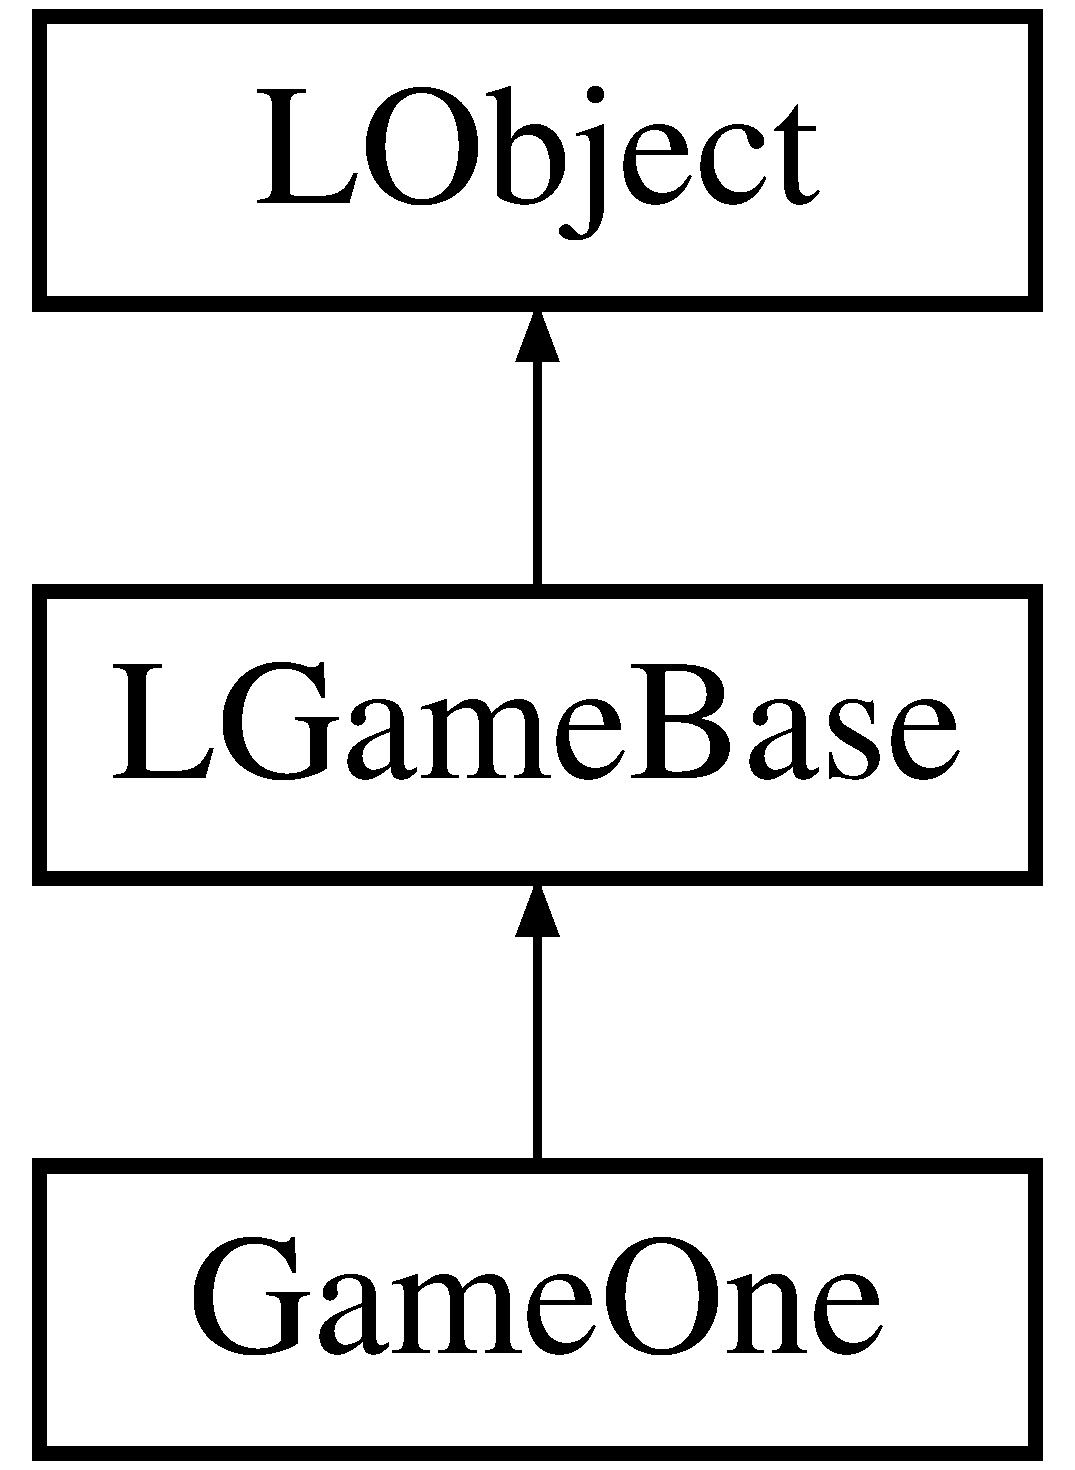
\includegraphics[height=3.000000cm]{class_game_one}
\end{center}
\end{figure}
\subsection*{Public Member Functions}
\begin{DoxyCompactItemize}
\item 
\hypertarget{class_game_one_a76590917f2525e502798d3a8b1916303}{virtual e\-Error {\bfseries Create} ()}\label{class_game_one_a76590917f2525e502798d3a8b1916303}

\item 
\hypertarget{class_game_one_accbd99a0a216c5e2437ffa89d698f356}{virtual e\-Error {\bfseries Initialise} ()}\label{class_game_one_accbd99a0a216c5e2437ffa89d698f356}

\item 
\hypertarget{class_game_one_ac389e6f73fe47ecff5db0b6c5b6b53e1}{virtual e\-Error {\bfseries Update} ()}\label{class_game_one_ac389e6f73fe47ecff5db0b6c5b6b53e1}

\item 
\hypertarget{class_game_one_a51bff7285daf69d4ceffa88313cd9ebf}{virtual e\-Error {\bfseries Reset} ()}\label{class_game_one_a51bff7285daf69d4ceffa88313cd9ebf}

\item 
\hypertarget{class_game_one_a0fb2af6516be1647500dc16ae2610630}{virtual e\-Error {\bfseries Destroy} ()}\label{class_game_one_a0fb2af6516be1647500dc16ae2610630}

\end{DoxyCompactItemize}
\subsection*{Additional Inherited Members}


The documentation for this class was generated from the following files\-:\begin{DoxyCompactItemize}
\item 
Source/include/Game\-One.\-h\item 
Source/src/Game\-One.\-cpp\end{DoxyCompactItemize}

\hypertarget{class_l_engine}{\section{L\-Engine Class Reference}
\label{class_l_engine}\index{L\-Engine@{L\-Engine}}
}
\subsection*{Public Member Functions}
\begin{DoxyCompactItemize}
\item 
\hypertarget{class_l_engine_ac9dbd4fedf25c42bb0e573e4c48d1eb9}{e\-Error {\bfseries init} ()}\label{class_l_engine_ac9dbd4fedf25c42bb0e573e4c48d1eb9}

\item 
\hypertarget{class_l_engine_af232ceca2cbf1e0d083e62ef32e4c9b5}{e\-Error {\bfseries run} ()}\label{class_l_engine_af232ceca2cbf1e0d083e62ef32e4c9b5}

\item 
\hypertarget{class_l_engine_a28aae4a58cc000859bee6da7e9352fe5}{e\-Error {\bfseries quit} ()}\label{class_l_engine_a28aae4a58cc000859bee6da7e9352fe5}

\end{DoxyCompactItemize}


The documentation for this class was generated from the following files\-:\begin{DoxyCompactItemize}
\item 
Source/\-Libraries/\-L\-Engine/include/L\-Engine.\-h\item 
Source/\-Libraries/\-L\-Engine/src/L\-Engine.\-cpp\end{DoxyCompactItemize}

\hypertarget{class_l_game_base}{\section{L\-Game\-Base Class Reference}
\label{class_l_game_base}\index{L\-Game\-Base@{L\-Game\-Base}}
}
Inheritance diagram for L\-Game\-Base\-:\begin{figure}[H]
\begin{center}
\leavevmode
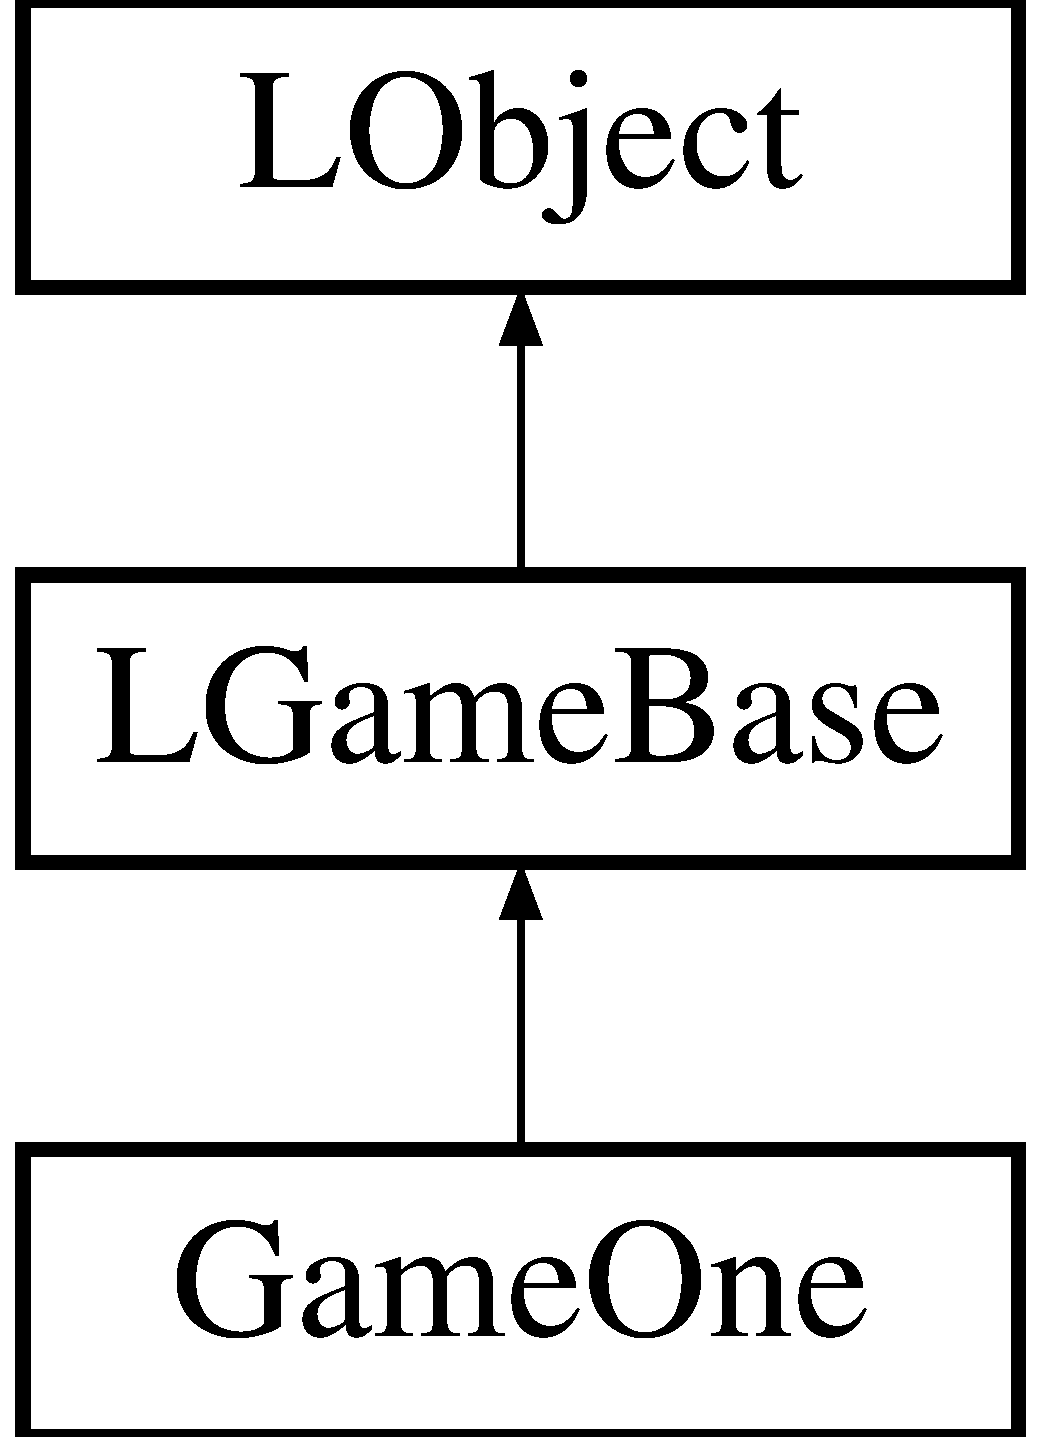
\includegraphics[height=3.000000cm]{class_l_game_base}
\end{center}
\end{figure}
\subsection*{Public Member Functions}
\begin{DoxyCompactItemize}
\item 
\hypertarget{class_l_game_base_a3365858f9e03e10b57a6e98b1c727814}{virtual e\-Error {\bfseries Create} ()}\label{class_l_game_base_a3365858f9e03e10b57a6e98b1c727814}

\item 
\hypertarget{class_l_game_base_a77672fe6db779dc83edec051c8c4dc32}{virtual e\-Error {\bfseries Initialise} ()}\label{class_l_game_base_a77672fe6db779dc83edec051c8c4dc32}

\item 
\hypertarget{class_l_game_base_ad45e09e8fee15456c145644f0efc0c88}{virtual e\-Error {\bfseries Update} ()}\label{class_l_game_base_ad45e09e8fee15456c145644f0efc0c88}

\item 
\hypertarget{class_l_game_base_a47c0cc5cb8f7cc4c733e5c1599db27c9}{virtual e\-Error {\bfseries Reset} ()}\label{class_l_game_base_a47c0cc5cb8f7cc4c733e5c1599db27c9}

\item 
\hypertarget{class_l_game_base_a741614c221d39efb8296d72f3011970b}{virtual e\-Error {\bfseries Destroy} ()}\label{class_l_game_base_a741614c221d39efb8296d72f3011970b}

\end{DoxyCompactItemize}
\subsection*{Static Public Member Functions}
\begin{DoxyCompactItemize}
\item 
\hypertarget{class_l_game_base_aeb53fd467d303a2fb78f1b4f0e8882df}{static \hyperlink{class_l_game_base}{L\-Game\-Base} $\ast$ {\bfseries Get\-Game} ()}\label{class_l_game_base_aeb53fd467d303a2fb78f1b4f0e8882df}

\end{DoxyCompactItemize}


The documentation for this class was generated from the following files\-:\begin{DoxyCompactItemize}
\item 
Source/\-Libraries/\-L\-Engine/include/L\-Game\-Base.\-h\item 
Source/\-Libraries/\-L\-Engine/src/L\-Game\-Base.\-cpp\item 
Source/src/Game\-One.\-cpp\end{DoxyCompactItemize}

\hypertarget{class_l_object}{\section{L\-Object Class Reference}
\label{class_l_object}\index{L\-Object@{L\-Object}}
}
Inheritance diagram for L\-Object\-:\begin{figure}[H]
\begin{center}
\leavevmode
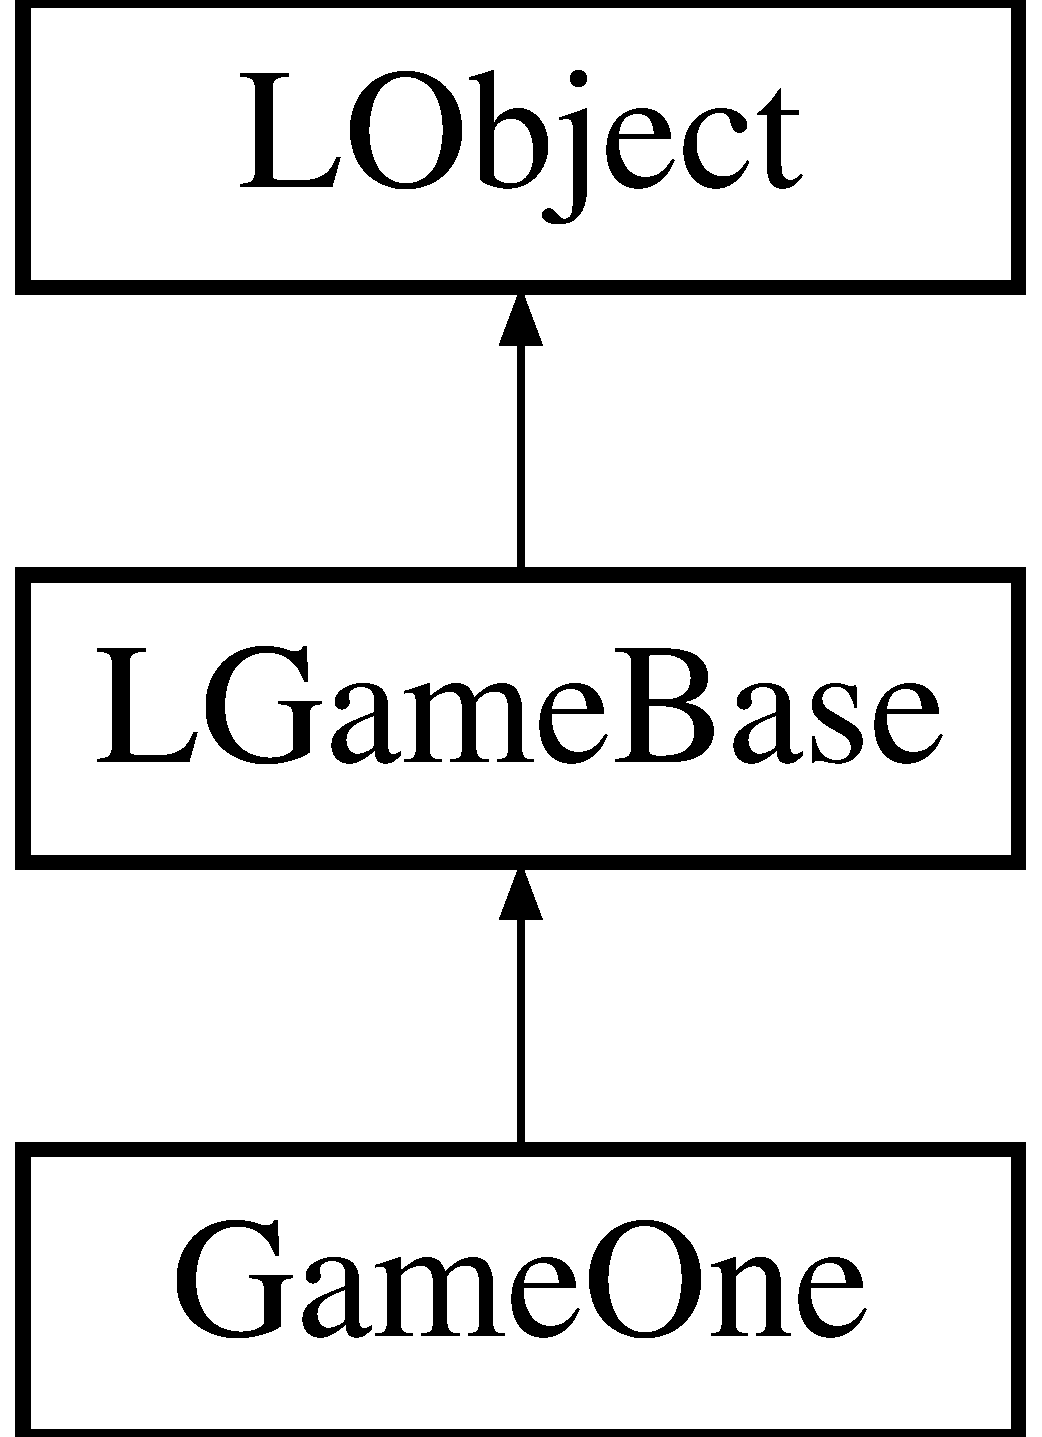
\includegraphics[height=3.000000cm]{class_l_object}
\end{center}
\end{figure}
\subsection*{Public Member Functions}
\begin{DoxyCompactItemize}
\item 
\hypertarget{class_l_object_a121190dfa412ad2d04900601cf5be9d8}{virtual e\-Error {\bfseries Create} ()=0}\label{class_l_object_a121190dfa412ad2d04900601cf5be9d8}

\item 
\hypertarget{class_l_object_aa7775558c54712e90d9f851d1069799d}{virtual e\-Error {\bfseries Initialise} ()=0}\label{class_l_object_aa7775558c54712e90d9f851d1069799d}

\item 
\hypertarget{class_l_object_a08a1f5faba2754f42e431d7b2a28fe95}{virtual e\-Error {\bfseries Update} ()=0}\label{class_l_object_a08a1f5faba2754f42e431d7b2a28fe95}

\item 
\hypertarget{class_l_object_ab8b747a026d8683c242d1a5c52ba6def}{virtual e\-Error {\bfseries Reset} ()=0}\label{class_l_object_ab8b747a026d8683c242d1a5c52ba6def}

\item 
\hypertarget{class_l_object_ac57da01b8d4eddd57d2fed543118e931}{virtual e\-Error {\bfseries Destroy} ()=0}\label{class_l_object_ac57da01b8d4eddd57d2fed543118e931}

\end{DoxyCompactItemize}


The documentation for this class was generated from the following file\-:\begin{DoxyCompactItemize}
\item 
Source/\-Libraries/\-L\-Engine/include/\hyperlink{_l_object_8h}{L\-Object.\-h}\end{DoxyCompactItemize}

\hypertarget{class_s_d_l_renderer}{\section{S\-D\-L\-Renderer Class Reference}
\label{class_s_d_l_renderer}\index{S\-D\-L\-Renderer@{S\-D\-L\-Renderer}}
}
\subsection*{Public Member Functions}
\begin{DoxyCompactItemize}
\item 
\hypertarget{class_s_d_l_renderer_a4e285fad6b9bf9d6d146950cf7f134ce}{e\-Error {\bfseries Create} (\hyperlink{class_s_d_l_window}{S\-D\-L\-Window} $\ast$window)}\label{class_s_d_l_renderer_a4e285fad6b9bf9d6d146950cf7f134ce}

\item 
\hypertarget{class_s_d_l_renderer_af04b495115d2d82e261978b790cbde6e}{e\-Error {\bfseries Render} ()}\label{class_s_d_l_renderer_af04b495115d2d82e261978b790cbde6e}

\item 
\hypertarget{class_s_d_l_renderer_a6555de3413ba1f4ea19a86df9f9b63b4}{e\-Error {\bfseries Destroy} ()}\label{class_s_d_l_renderer_a6555de3413ba1f4ea19a86df9f9b63b4}

\end{DoxyCompactItemize}


The documentation for this class was generated from the following files\-:\begin{DoxyCompactItemize}
\item 
Source/\-Libraries/\-S\-D\-L\-Interface/include/S\-D\-L\-Renderer.\-h\item 
Source/\-Libraries/\-S\-D\-L\-Interface/src/S\-D\-L\-Renderer.\-cpp\end{DoxyCompactItemize}

\hypertarget{class_s_d_l_window}{\section{S\-D\-L\-Window Class Reference}
\label{class_s_d_l_window}\index{S\-D\-L\-Window@{S\-D\-L\-Window}}
}
\subsection*{Public Member Functions}
\begin{DoxyCompactItemize}
\item 
\hypertarget{class_s_d_l_window_a745cd15bec2ad99813fb082f67896488}{e\-Error {\bfseries Create} ()}\label{class_s_d_l_window_a745cd15bec2ad99813fb082f67896488}

\item 
\hypertarget{class_s_d_l_window_a48f1ae5f9326fa006e8df73d4d0bd85f}{e\-Error {\bfseries Update} ()}\label{class_s_d_l_window_a48f1ae5f9326fa006e8df73d4d0bd85f}

\item 
\hypertarget{class_s_d_l_window_ab693926c16954fb9b6ec5cb0711ac117}{e\-Error {\bfseries Destroy} ()}\label{class_s_d_l_window_ab693926c16954fb9b6ec5cb0711ac117}

\end{DoxyCompactItemize}


The documentation for this class was generated from the following files\-:\begin{DoxyCompactItemize}
\item 
Source/\-Libraries/\-S\-D\-L\-Interface/include/S\-D\-L\-Window.\-h\item 
Source/\-Libraries/\-S\-D\-L\-Interface/src/S\-D\-L\-Window.\-cpp\end{DoxyCompactItemize}

\chapter{File Documentation}
\hypertarget{_game_one_8h}{\section{Source/include/\-Game\-One.h File Reference}
\label{_game_one_8h}\index{Source/include/\-Game\-One.\-h@{Source/include/\-Game\-One.\-h}}
}
{\ttfamily \#include \char`\"{}L\-Game\-Base.\-h\char`\"{}}\\*
\subsection*{Classes}
\begin{DoxyCompactItemize}
\item 
class \hyperlink{class_game_one}{Game\-One}
\end{DoxyCompactItemize}


\subsection{Detailed Description}
\begin{DoxyAuthor}{Author}
Marc Di luzio 
\end{DoxyAuthor}
\begin{DoxyDate}{Date}
April 2014
\end{DoxyDate}
Header for \hyperlink{_game_one_8cpp}{Game\-One.\-cpp} 
\hypertarget{_test_doxy_8h}{\section{Source/include/\-Test\-Doxy.h File Reference}
\label{_test_doxy_8h}\index{Source/include/\-Test\-Doxy.\-h@{Source/include/\-Test\-Doxy.\-h}}
}
\subsection*{Classes}
\begin{DoxyCompactItemize}
\item 
class \hyperlink{class_doxy_class}{Doxy\-Class}
\end{DoxyCompactItemize}


\subsection{Detailed Description}
\begin{DoxyAuthor}{Author}
\mbox{[}your name\mbox{]} 
\end{DoxyAuthor}
\begin{DoxyDate}{Date}
\mbox{[}the date\mbox{]}
\end{DoxyDate}
\mbox{[}detailed description\mbox{]} 
\hypertarget{_l_game_base_8h}{\section{Source/\-Libraries/\-L\-Engine/include/\-L\-Game\-Base.h File Reference}
\label{_l_game_base_8h}\index{Source/\-Libraries/\-L\-Engine/include/\-L\-Game\-Base.\-h@{Source/\-Libraries/\-L\-Engine/include/\-L\-Game\-Base.\-h}}
}
{\ttfamily \#include \char`\"{}types.\-h\char`\"{}}\\*
{\ttfamily \#include \char`\"{}L\-Object.\-h\char`\"{}}\\*
\subsection*{Classes}
\begin{DoxyCompactItemize}
\item 
class \hyperlink{class_l_game_base}{L\-Game\-Base}
\end{DoxyCompactItemize}


\subsection{Detailed Description}
\begin{DoxyAuthor}{Author}
Marc Di luzio 
\end{DoxyAuthor}
\begin{DoxyDate}{Date}
April 2014
\end{DoxyDate}
Header for \hyperlink{_l_game_base_8cpp}{L\-Game\-Base.\-cpp} 
\hypertarget{_l_object_8h}{\section{Source/\-Libraries/\-L\-Engine/include/\-L\-Object.h File Reference}
\label{_l_object_8h}\index{Source/\-Libraries/\-L\-Engine/include/\-L\-Object.\-h@{Source/\-Libraries/\-L\-Engine/include/\-L\-Object.\-h}}
}
\subsection*{Classes}
\begin{DoxyCompactItemize}
\item 
class \hyperlink{class_l_object}{L\-Object}
\end{DoxyCompactItemize}


\subsection{Detailed Description}
\begin{DoxyAuthor}{Author}
Marc Di luzio 
\end{DoxyAuthor}
\begin{DoxyDate}{Date}
April 2014
\end{DoxyDate}
Header for L\-Object.\-cpp 
\hypertarget{_l_game_base_8cpp}{\section{Source/\-Libraries/\-L\-Engine/src/\-L\-Game\-Base.cpp File Reference}
\label{_l_game_base_8cpp}\index{Source/\-Libraries/\-L\-Engine/src/\-L\-Game\-Base.\-cpp@{Source/\-Libraries/\-L\-Engine/src/\-L\-Game\-Base.\-cpp}}
}
{\ttfamily \#include \char`\"{}L\-Game\-Base.\-h\char`\"{}}\\*


\subsection{Detailed Description}
\begin{DoxyAuthor}{Author}
Marc Di luzio 
\end{DoxyAuthor}
\begin{DoxyDate}{Date}
April 2014
\end{DoxyDate}
Description 
\hypertarget{_s_d_l_event_loop_8h}{\section{Source/\-Libraries/\-S\-D\-L\-Interface/include/\-S\-D\-L\-Event\-Loop.h File Reference}
\label{_s_d_l_event_loop_8h}\index{Source/\-Libraries/\-S\-D\-L\-Interface/include/\-S\-D\-L\-Event\-Loop.\-h@{Source/\-Libraries/\-S\-D\-L\-Interface/include/\-S\-D\-L\-Event\-Loop.\-h}}
}
{\ttfamily \#include \char`\"{}types.\-h\char`\"{}}\\*
\subsection*{Functions}
\begin{DoxyCompactItemize}
\item 
\hypertarget{namespace_s_d_l_event_loop_ab9da5ad6897958f855e6babb41538ec1}{e\-Error {\bfseries S\-D\-L\-Event\-Loop\-::\-Do\-Loop} (bool \&exit)}\label{namespace_s_d_l_event_loop_ab9da5ad6897958f855e6babb41538ec1}

\item 
\hypertarget{namespace_s_d_l_event_loop_a901d2f2d5e402e04ac2dd25a2fee72be}{e\-Error {\bfseries S\-D\-L\-Event\-Loop\-::\-Handle\-Keyboard\-Event} (S\-D\-L\-\_\-\-Event $\ast$event)}\label{namespace_s_d_l_event_loop_a901d2f2d5e402e04ac2dd25a2fee72be}

\item 
\hypertarget{namespace_s_d_l_event_loop_a1ae5812e2e51c5d778dffc52ff0c925d}{e\-Error {\bfseries S\-D\-L\-Event\-Loop\-::\-Handle\-Joystick\-Event} (S\-D\-L\-\_\-\-Event $\ast$event)}\label{namespace_s_d_l_event_loop_a1ae5812e2e51c5d778dffc52ff0c925d}

\item 
\hypertarget{namespace_s_d_l_event_loop_ac54c96a30eee6bc633c5b82342a9ed11}{e\-Error {\bfseries S\-D\-L\-Event\-Loop\-::\-Handle\-Mouse\-Event} (S\-D\-L\-\_\-\-Event $\ast$event)}\label{namespace_s_d_l_event_loop_ac54c96a30eee6bc633c5b82342a9ed11}

\item 
\hypertarget{namespace_s_d_l_event_loop_a4a184f7106c67c0301cc67bd47b318a4}{e\-Error {\bfseries S\-D\-L\-Event\-Loop\-::\-Handle\-Controller\-Event} (S\-D\-L\-\_\-\-Event $\ast$event)}\label{namespace_s_d_l_event_loop_a4a184f7106c67c0301cc67bd47b318a4}

\end{DoxyCompactItemize}


\subsection{Detailed Description}
\begin{DoxyAuthor}{Author}
Marc Di luzio 
\end{DoxyAuthor}
\begin{DoxyDate}{Date}
April 2014
\end{DoxyDate}
Header for \hyperlink{_s_d_l_event_loop_8cpp}{S\-D\-L\-Event\-Loop.\-cpp} 
\hypertarget{_s_d_l_main_8h}{\section{Source/\-Libraries/\-S\-D\-L\-Interface/include/\-S\-D\-L\-Main.h File Reference}
\label{_s_d_l_main_8h}\index{Source/\-Libraries/\-S\-D\-L\-Interface/include/\-S\-D\-L\-Main.\-h@{Source/\-Libraries/\-S\-D\-L\-Interface/include/\-S\-D\-L\-Main.\-h}}
}
{\ttfamily \#include \char`\"{}types.\-h\char`\"{}}\\*
\subsection*{Functions}
\begin{DoxyCompactItemize}
\item 
\hypertarget{namespace_s_d_l_main_aed1793f23cba08927cbef5fdba20d8c7}{e\-Error {\bfseries S\-D\-L\-Main\-::\-Init} ()}\label{namespace_s_d_l_main_aed1793f23cba08927cbef5fdba20d8c7}

\item 
\hypertarget{namespace_s_d_l_main_aea08cc00b81235790cea0360fec763ac}{e\-Error {\bfseries S\-D\-L\-Main\-::\-Quit} ()}\label{namespace_s_d_l_main_aea08cc00b81235790cea0360fec763ac}

\end{DoxyCompactItemize}


\subsection{Detailed Description}
\begin{DoxyAuthor}{Author}
Marc Di luzio 
\end{DoxyAuthor}
\begin{DoxyDate}{Date}
April 2014
\end{DoxyDate}
Header for S\-D\-L\-Main.\-cpp 
\hypertarget{_s_d_l_window_8h}{\section{Source/\-Libraries/\-S\-D\-L\-Interface/include/\-S\-D\-L\-Window.h File Reference}
\label{_s_d_l_window_8h}\index{Source/\-Libraries/\-S\-D\-L\-Interface/include/\-S\-D\-L\-Window.\-h@{Source/\-Libraries/\-S\-D\-L\-Interface/include/\-S\-D\-L\-Window.\-h}}
}
{\ttfamily \#include \char`\"{}types.\-h\char`\"{}}\\*
\subsection*{Classes}
\begin{DoxyCompactItemize}
\item 
class \hyperlink{class_s_d_l_window}{S\-D\-L\-Window}
\end{DoxyCompactItemize}


\subsection{Detailed Description}
\begin{DoxyAuthor}{Author}
Marc Di luzio 
\end{DoxyAuthor}
\begin{DoxyDate}{Date}
April 2014
\end{DoxyDate}
Header for \hyperlink{_s_d_l_window_8cpp}{S\-D\-L\-Window.\-cpp} 
\hypertarget{_s_d_l_event_loop_8cpp}{\section{Source/\-Libraries/\-S\-D\-L\-Interface/src/\-S\-D\-L\-Event\-Loop.cpp File Reference}
\label{_s_d_l_event_loop_8cpp}\index{Source/\-Libraries/\-S\-D\-L\-Interface/src/\-S\-D\-L\-Event\-Loop.\-cpp@{Source/\-Libraries/\-S\-D\-L\-Interface/src/\-S\-D\-L\-Event\-Loop.\-cpp}}
}
{\ttfamily \#include \char`\"{}S\-D\-L\-Event\-Loop.\-h\char`\"{}}\\*
{\ttfamily \#include \char`\"{}S\-D\-L.\-h\char`\"{}}\\*


\subsection{Detailed Description}
\begin{DoxyAuthor}{Author}
Marc Di luzio 
\end{DoxyAuthor}
\begin{DoxyDate}{Date}
April 2014
\end{DoxyDate}
Description 
\hypertarget{_s_d_l_renderer_8cpp}{\section{Source/\-Libraries/\-S\-D\-L\-Interface/src/\-S\-D\-L\-Renderer.cpp File Reference}
\label{_s_d_l_renderer_8cpp}\index{Source/\-Libraries/\-S\-D\-L\-Interface/src/\-S\-D\-L\-Renderer.\-cpp@{Source/\-Libraries/\-S\-D\-L\-Interface/src/\-S\-D\-L\-Renderer.\-cpp}}
}
{\ttfamily \#include \char`\"{}S\-D\-L\-Renderer.\-h\char`\"{}}\\*


\subsection{Detailed Description}
\begin{DoxyAuthor}{Author}
Marc Di luzio 
\end{DoxyAuthor}
\begin{DoxyDate}{Date}
April 2014
\end{DoxyDate}
Description 
\hypertarget{_s_d_l_window_8cpp}{\section{Source/\-Libraries/\-S\-D\-L\-Interface/src/\-S\-D\-L\-Window.cpp File Reference}
\label{_s_d_l_window_8cpp}\index{Source/\-Libraries/\-S\-D\-L\-Interface/src/\-S\-D\-L\-Window.\-cpp@{Source/\-Libraries/\-S\-D\-L\-Interface/src/\-S\-D\-L\-Window.\-cpp}}
}
{\ttfamily \#include \char`\"{}S\-D\-L\-Window.\-h\char`\"{}}\\*
{\ttfamily \#include \char`\"{}S\-D\-L.\-h\char`\"{}}\\*


\subsection{Detailed Description}
\begin{DoxyAuthor}{Author}
Marc Di luzio 
\end{DoxyAuthor}
\begin{DoxyDate}{Date}
April 2014
\end{DoxyDate}
Description 
\hypertarget{_game_one_8cpp}{\section{Source/src/\-Game\-One.cpp File Reference}
\label{_game_one_8cpp}\index{Source/src/\-Game\-One.\-cpp@{Source/src/\-Game\-One.\-cpp}}
}
{\ttfamily \#include \char`\"{}Game\-One.\-h\char`\"{}}\\*


\subsection{Detailed Description}
\begin{DoxyAuthor}{Author}
Marc Di luzio 
\end{DoxyAuthor}
\begin{DoxyDate}{Date}
April 2014
\end{DoxyDate}
Main game class, responsible for managing all game specific stuff 
\hypertarget{main_8cpp}{\section{Source/src/main.cpp File Reference}
\label{main_8cpp}\index{Source/src/main.\-cpp@{Source/src/main.\-cpp}}
}
{\ttfamily \#include \char`\"{}stdio.\-h\char`\"{}}\\*
{\ttfamily \#include \char`\"{}types.\-h\char`\"{}}\\*
{\ttfamily \#include \char`\"{}L\-Engine.\-h\char`\"{}}\\*
\subsection*{Functions}
\begin{DoxyCompactItemize}
\item 
\hypertarget{main_8cpp_a700a0caa5b70a06d1064e576f9f3cf65}{int {\bfseries main} (int argc, char $\ast$args\mbox{[}$\,$\mbox{]})}\label{main_8cpp_a700a0caa5b70a06d1064e576f9f3cf65}

\end{DoxyCompactItemize}


\subsection{Detailed Description}
\begin{DoxyAuthor}{Author}
Marc Di luzio 
\end{DoxyAuthor}
\begin{DoxyDate}{Date}
April 2014
\end{DoxyDate}
Description 
%--- End generated contents ---

% Index
\newpage
\phantomsection
\addcontentsline{toc}{part}{Index}
\printindex

\end{document}
